\chapter{Introduction} \label{chap:Introduction}

\blindtext

\begin{figure}
    \centering
    \begin{adjustbox}{minipage=\dimexpr\textwidth-2\fboxsep-2\fboxrule,fbox}
        \begin{subfigure}[b]{0.475\textwidth}
            \caption[\textit{Alphainfluenzavirus}]{\textbf{\textit{Alphainfluenzavirus}}}
            \label{subfig:Influenza_A}
            \includegraphics[width=\textwidth]{Graphics/Influenza_A.pdf}
        \end{subfigure}
        \hfill
        \begin{subfigure}[b]{0.475\textwidth}
            \caption[\textit{Betainfluenzavirus}]{\textbf{\textit{Betainfluenzavirus}}}
            \label{subfig:Influenza_B}
            \includegraphics[width=\textwidth]{Graphics/Influenza_B.pdf}
        \end{subfigure}
    \end{adjustbox}
    \caption[\textit{Orthomyxoviridae}]{\textbf{\textit{Orthomyxoviridae}.} .}
    \label{fig:Orthomyxoviridae}
\end{figure}

\begin{figure}
    \centering
    \begin{adjustbox}{minipage=\dimexpr\textwidth-2\fboxsep-2\fboxrule,fbox}
        \begin{subfigure}[b]{0.475\textwidth}
            \caption[Euclidean]{\textbf{Euclidean}}
            \label{subfig:Euclidean}
            \includegraphics[width=\textwidth]{Graphics/Euclidean.pdf}
        \end{subfigure}
        \hfill
        \begin{subfigure}[b]{0.475\textwidth}
            \caption[Cosine]{\textbf{Cosine}}
            \label{subfig:Cosinus}            \includegraphics[width=\textwidth]{Graphics/Cosinus.pdf}
        \end{subfigure}
    \end{adjustbox}
    \caption[Distance Measuring Methods]{\textbf{Distance Measuring Methods.} .}
    \label{fig:Distance}
\end{figure}

\blindtext

\begin{figure}
    \centering
    \begin{adjustbox}{minipage=\dimexpr\textwidth-2\fboxsep-2\fboxrule,fbox}
        \begin{subfigure}[b]{0.475\textwidth}
            \caption[Compactness]{\textbf{Compactness}}
            \label{subfig:Compactness}            \includegraphics[width=\textwidth]{Graphics/Compactness.pdf}
        \end{subfigure}
        \hfill
        \begin{subfigure}[b]{0.475\textwidth}
            \caption[Connectedness]{\textbf{Connectedness}}
            \label{subfig:Connectedness}            \includegraphics[width=\textwidth]{Graphics/Connectedness.pdf}
        \end{subfigure}
    \end{adjustbox}
    \caption[Clustering Methods]{\textbf{Clustering Methods.} .}
    \label{fig:Methods}
\end{figure}

\blindtext